\documentclass{article}
\usepackage[utf8]{inputenc}
\usepackage{graphicx}


\title{Tecnologías semánticas}
\author{Noelia Fernández Salmerón }

\begin{document}
\maketitle
\begin{abstract}
https://github.com/Noeliafs/proyectofinal\\
Este es nuestro primer artículo científico para el curso {\bf LaTeX y Git aplicado a la investigación científica}. En él vamos a tratar aspectos relacionados con las tecnologías semánticas, principalmente las ontologías.
\end{abstract}
\section{Introducción}
La organización del conocimiento y la recuperación de la información han sido objeto de estudio en diversos campos. Su base principal es el conocimiento, el cual es una combinación de información, procedimientos y conexiones que implica el procesamiento racional y reflexivo de la información, además del desarrollo de procesos que involucran, por un lado, la discriminación entre información relevante y no relevante teniendo en cuenta unos intereses establecidos previamente, y por el otro, una reflexión que propicia la deconstrucción y reconstrucción de mensajes a partir de una
realidad (personal, social, cultural, etc.) 


\section{Estado del arte}
\subsection{Web semántica}
Como antes hemos comentado, la Web Semántica es una visión para el futuro de la Web en la que se da información de significado explícito, por lo que es más fácil para las máquinas procesar de forma automática e integrar la información disponible en la Web. Uno de los pioneros de la web semántica fue Tim Berners-Lee, el cuál suponía que en la web de un futuro los ordenadores podrían acceder a información que estuviera semánticamente marcada y estructurada mediante ontologías que expresarían tanto conceptos como conjuntos de reglas de inferencias útiles con el objetivo de llevar a cabo razonamientos automáticos sobre las páginas web para que los ordenadores pudieran desarrollar tareas inteligentes. En la siguiente tabla se resume la evolución de la web.

\begin{table}[h]
\centering
\begin{tabular}{c c c} 
%nùmero de columnas: 3
Web & Unidireccional/Bidireccional & Estática/Dinámica \\ \hline
Web 1.0 & Unidireccional, sólo lectura & Estática\\
Web 1.x & Unidireccional, sólo lectura & Aporta dinamismo \\
Web 2.0 & Bidireccional (colaboración) & Dinámica (redes sociales)\\
Web 3.0 & Totalmente colaborativa & Tecnología de la inteligencia artificial 
\end{tabular}
\caption{\label{tab:tabla ejemplo}Evolución de la web.}
\end{table}

\subsection{Lenguajes y herramientas software}
En el año 2000, Tim Berners-Lee propuso un modelo esquematizado dónde se pueden apreciar los diferentes lenguajes que se utilizan en la web semántica. Berners-Lee nombró este esquema como Semantic Web Layer Cake, como puede apreciarse en la Figura 1.


\begin{figure}[h]
\centering
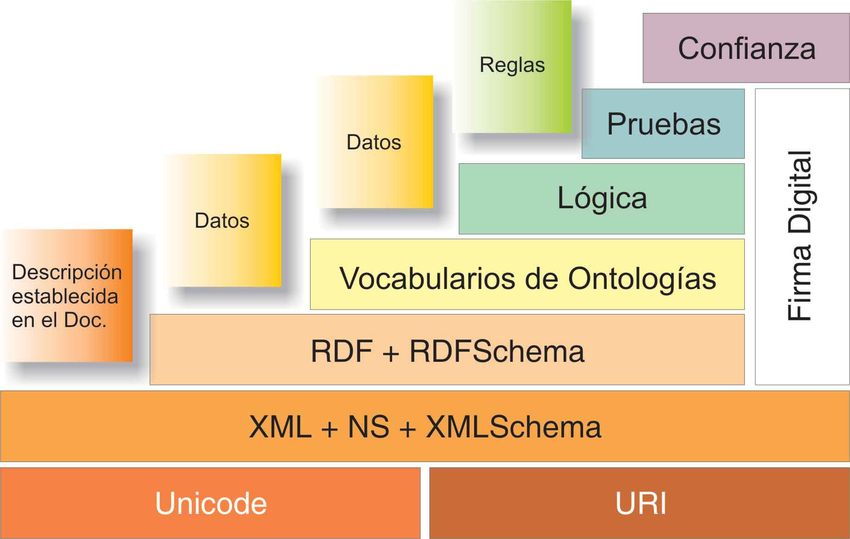
\includegraphics[width=0.6\textwidth]{imagenes/modelo_capas.png}
\caption{\label{fig:modelo_capas}Capas de la Web Semántica.}
\end{figure}

\section{Objetivos}
\begin{enumerate}
    \item Conocer el estado del arte de las tecnologías semánticas.
    \item Ventajas e incovenientes de su uso.
    \item Ejemplos en diferentes estudios.
\end{enumerate}

\section{Metodología}
\begin{enumerate}
    \item Formulación de hipótesis.
    \item Recogida de observaciones.
    \item Readaptación de las hipótesis iniciales a la luz de los resultados obtenidos.
\end{enumerate}

\section{Conclusiones}
Para finalizar este artículo vamos a añadir 


\section{Bibliografía}




\end{document}
